\begin{tabular}{M{6.5cm}M{11cm}}
	\textbf{LỚP CÔ THẢO - THẦY SANG}& \textbf{ĐỀ ÔN TẬP KIỂM TRA CUỐI HỌC KÌ 1}\\
	\textbf{MÃ ĐỀ: 002}& \textbf{Bài thi môn: VẬT LÝ 12}\\
	\textit{(Đề trường THPT Lương Thế Vinh - Hà Nội năm học 2024 -2025)}& \textit{Thời gian làm bài: 50 phút, không kể thời gian phát đề}
	
	\noindent\rule{4cm}{0.8pt} \\
\end{tabular}
\setcounter{section}{0}
\section{Câu trắc nghiệm nhiều phương án lựa chọn}
\textit{Thí sinh trả lời từ câu 1 đến câu 18. Mỗi câu hỏi thí sinh chọn một phương án}
\setcounter{ex}{0}
\Opensolutionfile{ans}[ans/FINAL-SEM1-002-TN]
% ===================================================================
\begin{ex}
	Trong các chất sau, chất nào \textbf{không phải} là chất rắn kết tinh
	\choice
	{muối ăn}
	{\True thủy tinh}
	{kim cương}
	{thạch anh}
	\loigiai{}
\end{ex}
% ===================================================================
\begin{ex}
	Đặc điểm nào sau đây là đặc điểm của thể lỏng?
	\choice
	{Khoảng cách giữa các phân tử rất lớn so với kích thước của chúng}
	{\True Lực tương tác phân tử yếu hơn lực tương tác phân tử ở thể rắn}
	{Không có thể tích và hình dạng riêng xác định}
	{Các phân tử dao động xung quanh vị trí cân bằng xác định}
	\loigiai{}
\end{ex}
% ===================================================================
\begin{ex}
	Khi quan sát sự nóng chảy của nước đá tại nhiệt độ nóng chảy, trong suốt thời gian nóng chảy thì
	\choice
	{nhiệt độ của nước đá tăng}
	{nhiệt độ của nước đá giảm}
	{\True nhiệt độ của nước không thay đổi}
	{nhiệt độ của nước đá ban đầu tăng sau đó giảm}
	\loigiai{}
\end{ex}
% ===================================================================
\begin{ex}
	Sử dụng hai nhiệt kế rượu có độ chia từ $\SI{0}{\celsius}$ tới $\SI{100}{\celsius}$, hình vẽ nào trong hình bên dưới phù hợp với trường hợp nhiệt kế 1 được đặt vào một cốc đựng nước nóng còn nhiệt kế 2 được đặt vào một cốc nước lạnh?
	\begin{center}
		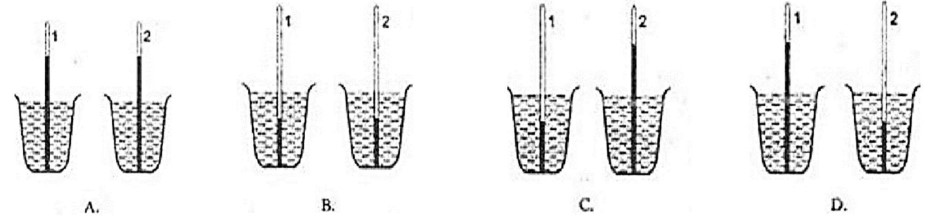
\includegraphics[scale=0.7]{../figs/FINAL-SEM1-002-1}
	\end{center}
	\choice
	{Hình B}
	{Hình C}
	{Hình A}
	{\True Hình D}
	\loigiai{}
\end{ex}
% ===================================================================
\begin{ex}
	\immini{Hiện tượng quả bóng bàn bị móp (nhưng chưa bị thủng) khi thả vào cốc nước nóng sẽ phồng trở lại là do nội năng của chất khí bên trong quả bóng}	
	{\vspace{-0.5cm}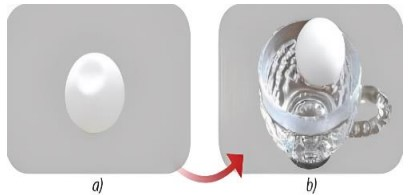
\includegraphics[scale=0.5]{../figs/FINAL-SEM1-002-2}}
	\choice
	{\True tăng lên}
	{giảm xuống}
	{không thay đổi}
	{giảm đi hai lần}
	\loigiai{}
\end{ex}
% ===================================================================
\begin{ex}
	Theo định luật I nhiệt động lực học $\Delta U=Q+A$. Biểu thức nào sau đây diễn tả quá trình biến thiên nội năng khi hệ nhận công và truyền nhiệt
	\choice
	{$\Delta U=Q+A$ với $Q>0$ và $A>0$}
	{$\Delta U=Q+A$ với $Q>0$ và $A<0$}
	{\True $\Delta U=Q+A$ với $Q<0$ và $A>0$}
	{$\Delta U=Q+A$ với $Q<0$ và $A<0$}
	\loigiai{}
\end{ex}
% ===================================================================
\begin{ex}
	Biết nhiệt nóng chảy riêng của nước đá là $\lambda=\SI{3.4E5}{\joule/\kilogram}$. Nhiệt lượng $Q$ cần cung cấp để làm nóng chảy $\SI{200}{\gram}$ nước đá ở $\SI{0}{\celsius}$ bằng
	\choice
	{$\SI{0.34E3}{\joule}$}
	{$\SI{340E5}{\joule}$}
	{$\SI{68E7}{\joule}$}
	{\True $\SI{68E3}{\joule}$}
	\loigiai{}
\end{ex}
% ===================================================================
\begin{ex}
	Biết nhiệt hóa hơi riêng của nước là $L=\SI{2.3E6}{\joule/\kilogram}$. Nhiệt lượng cần cung cấp để làm bay hơi hoàn toàn $\SI{300}{\gram}$ nước ở $\SI{100}{\celsius}$ là 
	\choice
	{$\SI{69E6}{\joule}$}
	{\True $\SI{6.9E5}{\joule}$}
	{$\SI{2.3E6}{\joule}$}
	{$\SI{0.23E4}{\joule}$}
	\loigiai{}
\end{ex}
% ===================================================================
\begin{ex}
\immini{Đồ thị biểu diễn hai đường đẳng nhiệt của cùng một lượng khí lí tưởng biểu diễn như hình vẽ. Mối quan hệ về nhiệt độ của hai đường đẳng nhiệt này là
	\choice
	{\True $T_2>T_1$}
	{$T_2=T_1$}
	{$T_2<T_1$}
	{$T_2\le T_1$}}
{\vspace{-0.5cm}	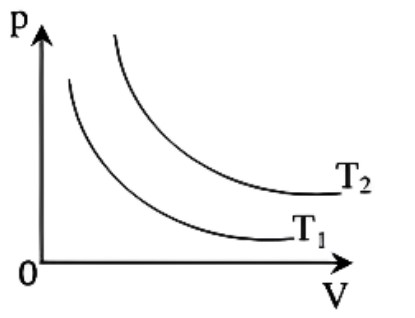
\includegraphics[scale=0.4]{../figs/FINAL-SEM1-002-3}}
	\loigiai{}
\end{ex}
% ===================================================================
\begin{ex}
	Một lượng khí có áp suất $\SI{750}{\milli\meter Hg}$, nhiệt độ $\SI{37}{\celsius}$ và thể tích $\SI{70}{\centi\meter^3}$. Thể tích khí ở điều kiện tiêu chuẩn (nhiệt độ $\SI{0}{\celsius}$ và áp suất $\SI{760}{\milli\meter Hg}$) có giá trị gần bằng
	\choice
	{$\SI{22.4}{\centi\meter^3}$}
	{$\SI{32.7}{\centi\meter^3}$}
	{\True $\SI{60.8}{\centi\meter^3}$}
	{$\SI{78}{\centi\meter^3}$}
	\loigiai{
	$\dfrac{p_1V_1}{T_1}=\dfrac{p_2V_2}{T_2}\Leftrightarrow\dfrac{750\cdot70}{37+273}=\dfrac{760V}{273}\Rightarrow V\approx\SI{60.8}{\centi\meter^3}$.
	}
\end{ex}
% ===================================================================
\begin{ex}
Gọi $p$ là áp suất khối khí, $\mu$ là mật độ của phân tử khí, $m$ là khối lượng của phân tử khí, $\overline{v^2}$ là trung bình của bình phương tốc độ, $k$ là hằng số Boltzmann, $T$ là nhiệt độ tuyệt đối. Công thức nào sau đây mô tả đúng mối liên hệ giữa các đại lượng?	
	\choice
	{$p=\dfrac{2}{3}\mu m\overline{v^2}$}
	{$p=3\mu kT$}
	{\True $p=\mu kT$}
	{$p=\dfrac{3}{2}\mu m\overline{v^2}$}
	\loigiai{}
\end{ex}
% ===================================================================
\begin{ex}
Động năng tịnh tiến trung bình của phân tử khí lí tưởng ở $\SI{37}{\celsius}$ có giá trị là	
	\choice
	{$\SI{5.21E-22}{\joule}$}
	{\True $\SI{6.42E-21}{\joule}$}
	{$\SI{6.24E23}{\joule}$}
	{$\SI{5.12E23}{\joule}$}
	\loigiai{
	$W_{\text{đ}}=\dfrac{3}{2}kT=\SI{6.42E-21}{\joule}.$
	}
\end{ex}
% ===================================================================
\begin{ex}
	Hình vẽ nào dưới đây biểu diễn đúng hướng của vector cảm ứng từ tại M gây ra bởi dòng điện trong dây dẫn thẳng dài vô hạn?
	\choice
	{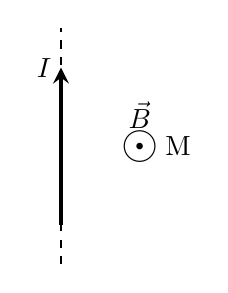
\begin{tikzpicture}
			\draw[dashed] (0,0)--(0,3);
			\draw[-stealth, line width=1.5pt] (0,0.5)--(0,2.5);
			\node at (1,1.5) {\LARGE $\odot$};
			\node[above] at (1,1.6) {$\vec{B}$};
			\node[left] at (0,2.5) {$I$};
			\node[right] at (1.2,1.5) {M};
	\end{tikzpicture}}
	{\True 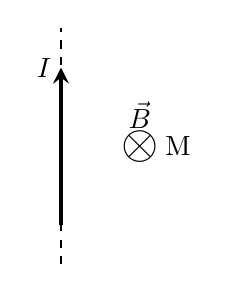
\begin{tikzpicture}
			\draw[dashed] (0,0)--(0,3);
			\draw[-stealth, line width=1.5pt] (0,0.5)--(0,2.5);
			\node at (1,1.5) {\LARGE $\otimes$};
			\node[above] at (1,1.6) {$\vec{B}$};
			\node[left] at (0,2.5) {$I$};
			\node[right] at (1.2,1.5) {M};
	\end{tikzpicture}}
	{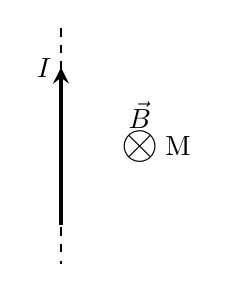
\begin{tikzpicture}
			\draw[dashed] (0,3)--(0,0);
			\draw[-stealth, line width=1.5pt] (0,0.5)--(0,2.5);
			\node at (1,1.5) {\LARGE $\otimes$};
			\node[above] at (1,1.6) {$\vec{B}$};
			\node[left] at (0,2.5) {$I$};
			\node[right] at (1.2,1.5) {M};
	\end{tikzpicture}}
	{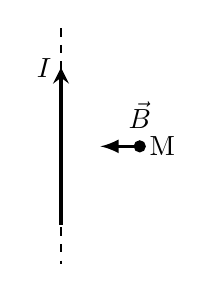
\begin{tikzpicture}
			\draw[dashed] (0,3)--(0,0);
			\draw[-stealth, line width=1.5pt] (0,0.5)--(0,2.5);
			\draw[-latex, line width=1.25pt] (1,1.5)--(0.5,1.5);
			\node[above] at (1,1.6) {$\vec{B}$};
			\node[left] at (0,2.5) {$I$};
			\filldraw (1,1.5) circle (2pt) node[right]{M};
	\end{tikzpicture}}
	\loigiai{}
\end{ex}
% ===================================================================
\begin{ex}
Hình nào sau đây biểu diễn không đúng vector lực từ tác dụng đoạn dây dẫn mang dòng điện đặt trong từ trường đều	
\begin{center}
	\begin{tabular}{M{4cm}M{4cm}M{4cm}M{4cm}}
		\begin{tikzpicture}
			\coordinate(A) at(0.2,0.2);
			\coordinate(B) at($(A)+(30:2.5)$);
			\foreach \x in {0,2}{
				\foreach \y in {0,2}{
					\node at (\x,\y) {\LARGE$\otimes$};
				}
			};
			\draw[-stealth, line width=1.5pt, blue] ($(A)!0.5!(B)$)--+(120:1.5);
			\draw[line width=4pt, gray,decoration={markings, mark=at position 0.5 with {\arrow{stealth}}},
			postaction={decorate}] (A)--(B);
			\node[below] at ($(A)!0.5!(B)$) {$I$};
			\node[right, blue] at ($(A)!0.5!(B)+(120:1.5)$) {$\vec{F}$};
			\node[right] at (2.1,2) {$\vec{B}$};
		\end{tikzpicture}
		&
		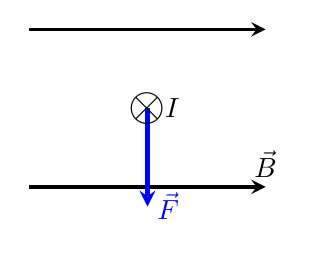
\begin{tikzpicture}
			\draw[-stealth, line width=1.25pt] (0,0)--(3,0);
			\draw[-stealth, line width=1.25pt] (0,2)--(3,2);
			\draw[-stealth, blue, line width=1.5pt] (1.5,1)--(1.5,-0.25);
			\node at(1.5,1) {\LARGE$\otimes$};
			\node[right] at(1.6,1) {$I$};
			\node[right, blue] at(1.5,-0.25) {$\vec{F}$};
			\node[above] at(3,0) {$\vec{B}$};
		\end{tikzpicture}
		&
		\begin{tikzpicture}
			\draw[-stealth, line width=1.25pt] (0,0)--(3,0);
			\draw[-stealth, line width=1.25pt] (0,2)--(3,2);
			\draw[-stealth, blue, line width=1.5pt] (1.5,1)--(1.5,2.25);
			\draw[line width=4pt, gray,decoration={markings, mark=at position 0.5 with {\arrow{stealth}}},
			postaction={decorate}] (0.5,1)--(2.5,1);
			\node[below] at(1.6,1) {$I$};
			\node[right, blue] at(1.5,2.25) {$\vec{F}$};
			\node[above] at(3,0) {$\vec{B}$};
		\end{tikzpicture}
		&
		\begin{tikzpicture}
			\coordinate(A) at (0.2,-0.2);
			\coordinate(B) at ($(A)+(-30:2.5)$);
			\draw[-stealth, line width=1.25pt] (0,0)--(0,-2);
			\draw[-stealth, line width=1.25pt] (2.5,0)--(2.5,-2);
			\draw[line width=4pt, gray,decoration={markings, mark=at position 0.5 with {\arrow{stealth}}},
			postaction={decorate}] (A)--(B);
			\node[above] at($(A)!0.5!(B)+(0,0.1)$) {$I$};
			\node[below, blue] at($(A)!0.5!(B)-(0,0.2)$) {$\vec{F}$};
			\node[above] at(3,0) {$\vec{B}$};
			\node[fill=none] at ($(A)!0.5!(B)$) {\LARGE$\otimes$};
		\end{tikzpicture}\\
		\textbf{Hình 1} & \textbf{Hình 2} & \textbf{Hình 3} & \textbf{Hình 4}
	\end{tabular}
\end{center}
	\choice
	{Hình 1}
	{Hình 2}
	{\True Hình 3}
	{Hình 4}
	\loigiai{}
\end{ex}
% ===================================================================
\begin{ex}
Một quả bóng có dung tích $\SI{2.5}{\liter}$. Người ta bơm không khí ở áp suất $\SI{E5}{\pascal}$ vào bóng. Mỗi lần bơm được $\SI{150}{\centi\meter^3}$ không khí. Tính áp suất của không khí trong quả bóng sau 50 lần bơm. Coi quả bóng trước khi bơm không có không khí và nhiệt độ trong quả bóng không thay đổi.
	\choice
	{$\SI{25E5}{\pascal}$}
	{$\SI{2.5E5}{\pascal}$}
	{$\SI{0.25E5}{\pascal}$}
	{\True $\SI{3E5}{\pascal}$}
	\loigiai{
	$p_1V_1=p_2V_2\Leftrightarrow10^5\cdot0,15\cdot50=2,5p\Rightarrow p=\SI{3E5}{\pascal}$.
	}
\end{ex}
% ===================================================================
\begin{ex}
	Ba chất lỏng không tác dụng hóa học với nhau và được trộn lẫn vào nhau trong một nhiệt lượng kế; chúng có khối lượng lần lượt là $m_1=\SI{1}{\kilogram}$, $m_2=\SI{10}{\kilogram}$, $m_3=\SI{5}{\kilogram}$ có nhiệt dung riêng lần lượt là $c_1=\SI{2000}{\kilogram\cdot\kelvin}$; $c_2=\SI{4000}{\joule/\kilogram\cdot\kelvin}$; $c_3=\SI{2500}{\joule/\kilogram\cdot\kelvin}$ và có nhiệt độ là $t_1=\SI{6}{\celsius}$; $t_2=\SI{20}{\celsius}$; $t_3=\SI{-60}{\celsius}$. Bỏ qua sự trao đổi nhiệt với nhiệt lượng kế và với môi trường. Nhiệt độ của hỗn hợp khi xảy ra cân bằng nhiệt xấp xỉ
	\choice
	{$\SI{-2.5}{\celsius}$}
	{$\SI{-1.9}{\celsius}$}
	{\True $\SI{1.1}{\celsius}$}
	{$\SI{3.5}{\celsius}$}
	\loigiai{
	$t_{\text{cb}}=\dfrac{m_1c_1t_1+m_2c_2t_2+m_3c_3t_3}{m_1c_1+m_2c_2+m_3c_3}\approx\SI{1.1}{\celsius}$.
	}
\end{ex}
% ===================================================================
\begin{ex}
	Khí helium có khối lượng mol phân tử là $\SI{4}{\gram/\mole}$. Coi các phân tử khí là giống nhau. Trung bình của bình phương tốc độ trong chuyển động nhiệt của phân tử khí helium ở nhiệt độ $\SI{320}{\kelvin}$ là
	\choice
	{$\SI{1.995E6}{\meter^2/\second^2}$}
	{$\SI{2.01E6}{\meter^2/\second^2}$}
	{$\SI{2010}{\meter^2/\second^2}$}
	{$\SI{2020}{\meter^2/\second^2}$}
	\loigiai{
	$\overline{v^2}=\dfrac{3RT}{M}\approx\SI{1.995E6}{\meter^2/\second^2}$.
	}
\end{ex}
% ===================================================================
\begin{ex}
	Treo đoạn dây dẫn có chiều dài $\ell=\SI{10}{\centi\meter}$, khối lượng $m=\SI{5}{\gram}$ bằng hai dây mảnh, nhẹ sao cho dây dẫn nằm ngang. Biết cảm ứng từ của từ trường hướng thẳng đứng xuống dưới, có độ lớn $B=\SI{0.5}{\tesla}$ và dòng điện đi qua dây dẫn là $I=\SI{1}{\ampere}$. Lấy $g=\SI{10}{\meter/\second^2}$ thì góc lệch của dây treo so với phương thẳng đứng là
	\choice
	{$\SI{30}{\degree}$}
	{\True $\SI{45}{\degree}$}
	{$\SI{60}{\degree}$}
	{$\SI{90}{\degree}$}
	\loigiai{
	$\tan\alpha=\dfrac{F}{P}=\dfrac{ILB}{mg}=1\Rightarrow \alpha=\SI{45}{\degree}$.
	}
\end{ex}
\Closesolutionfile{ans}
\section{Câu trắc nghiệm đúng/sai} 
\textit{Thí sinh trả lời từ câu 1 đến câu 4. Trong mỗi ý \textbf{a)}, \textbf{b)}, \textbf{c)}, \textbf{d)} ở mỗi câu, thí sinh chọn đúng hoặc sai}
\setcounter{ex}{0}
\Opensolutionfile{ans}[ans/FINAL-SEM1-002-TF]
% ===================================================================
\begin{ex}
	\immini{Cho đồ thị biểu diễn sự thay đổi nhiệt độ của nước theo thời gian đun như hình bên. Biết nhiệt độ nóng chảy của nước đá là $\SI{0}{\celsius}$, nhiệt độ sôi của nước là $\SI{100}{\celsius}$.
	\choiceTF[t]
	{\True Từ phút thứ 0 đến phút thứ 5 nước ở thể rắn}
	{\True Từ phút thứ 5 đến phút thứ 10 xảy ra quá trình nóng chảy}
	{Từ phút thứ 10 đến phút thứ 25 nước ở thể rắn}
	{\True Từ phút thứ 25 đến phút thứ 30 xảy ra quá trình sôi}
	}
	{\begin{tikzpicture}  
			\begin{axis}[  ultra thick,scale=0.65,
				xmin=0,  
				xmax=34,  
				xtick={0,5,...,35},
				ytick={-10,0,...,120},
				minor x tick num=1,
				minor y tick num=0,
				ymin=-10,  
				ymax=110, 
				samples=300,
				yticklabels=\empty,
				axis lines=center, 
				grid style={step=1, line width=0.8pt,gray!60!white},
				grid=both, %giới hạn ô lưới
				major grid style={line width=0.8pt,gray!60!white},
				xlabel=$\xsi{t}{\left(\minute\right)}$, 		
				ylabel=$\text{Nhiệt độ}\ \left(\si{\celsius}\right)$,
				every axis y label/.style={at=(current axis.above origin),anchor=south},  
				every axis x label/.style={at=(current axis.right of origin),anchor=south},  ]
				\coordinate (A) at (axis cs: 0,-10);
				\coordinate (B) at (axis cs: 5,0);
				\coordinate (C) at (axis cs: 10,0);
				\coordinate (D) at (axis cs: 25,100);
				\coordinate (E) at (axis cs: 30,100);
				\draw[line width=1.5pt,blue] plot coordinates {(A) (B) (C) (D) (E)};
				\coordinate (O) at (axis cs: 0,0);
				\coordinate (t1) at (axis cs: 0,-10);
				\coordinate (t2) at (axis cs: 0,100);
			\end{axis}  
			\node[left] at (O) {0};
			\node[left] at (t1) {$-10$};
			\node[left] at (t2) {$100$};
	\end{tikzpicture}}
	
	\loigiai{}
\end{ex}
% ===================================================================
\begin{ex}
\immini{Cung cấp nhiệt lượng $\SI{2.5}{\joule}$ cho một khối khí lí trong một xilanh đặt nằm ngang như hình vẽ. Chất khí nở ra đẩy pít-tông đi một đoạn $\SI{5.0}{\centi\meter}$. Biết lực ma sát giữa pít-tông và xilanh có độ lớn là $\SI{20.0}{\newton}$, diện tích tiết diện của pít-tông là $\SI{2.0}{\centi\meter^2}$. Coi pít-tông chuyển động thẳng đều và áp suất bên phải pít-tông bằng 0. Trong các phát biểu sau, phát biểu nào đúng, phát biểu nào sai?}
{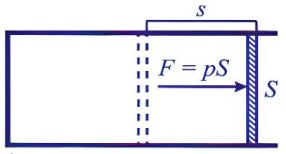
\includegraphics[scale=0.7]{../figs/FINAL-SEM1-002-4}}
	\choiceTF[t]
	{\True Công của khối khí thực hiện là $\SI{1.0}{\joule}$}
	{Độ biến thiên nội năng của khối khí là $\SI{0.50}{\joule}$}
	{\True Trong quá trình dãn nở, áp suất của chất khí là $\SI{1.0E5}{\pascal}$}
	{Thể tích khí trong xilanh tăng $\SI{5.0}{\liter}$}
	\loigiai{
	\begin{itemchoice}
		\itemch Đúng. $A'=Fs=\SI{1}{\joule}$.
		\itemch Sai. $\Delta U=Q-A'=\SI{1.5}{\joule}$.
		\itemch Đúng. $p=\dfrac{F}{S}=\SI{E5}{\pascal}$.
		\itemch Sai. $A'=p\Delta V\Rightarrow \Delta V=\SI{0.01}{\liter}$.
	\end{itemchoice}
	}
\end{ex}
% ===================================================================
\begin{ex}
	Một hệ làm nóng nước bằng năng lượng mặt trời có hiệu suất chuyển đổi $\SI{25}{\percent}$; cường độ bức xạ mặt trời lên bộ thu nhiệt là $\SI{1000}{\watt/\meter^2}$; diện tích bộ thu là $\SI{5}{\meter^2}$. Cho nhiệt dung riêng của nước là $\SI{4200}{\joule/\kilogram\cdot\kelvin}$.
	\choiceTF[t]
	{\True Công suất bức xạ chiếu lên bộ thu nhiệt là $\SI{5000}{\watt}$}
	{\True Trong $\SI{1.00}{\hour}$, năng lượng mặt trời chiếu lên bộ thu nhiệt là $\SI{18}{\mega\joule}$}
	{Trong $\SI{1.00}{\hour}$, phần năng lượng chuyển thành năng lượng nhiệt là $\SI{5}{\mega\joule}$}
	{Nếu hệ thống đó làm nóng $\SI{30.0}{\kilogram}$ nước thì trong khoảng thời gian $\SI{1.00}{\hour}$ nhiệt độ của nước tăng thêm $\SI{30}{\celsius}$}
	\loigiai{\begin{itemchoice}
			\itemch Đúng. $\calP=IS=\SI{5}{\kilo\watt}$.
			\itemch Đúng. $A=\calP t=\SI{18}{\mega\joule}$.
			\itemch Sai. $Q=HA=\SI{4.5}{\mega\joule}$.
			\itemch Sai. $\Delta t=\dfrac{Q}{mc}=\SI{35.7}{\celsius}$.
	\end{itemchoice}}
\end{ex}
% ===================================================================
\begin{ex}
	Có $\SI{16}{\gram}$ khí oxygen ở nhiệt độ $\SI{27}{\celsius}$, áp suất $\SI{3E5}{\pascal}$. Sau khi đun nóng đẳng áp, khối khí có thể tích là $\SI{10}{\liter}$. Biết khối lượng mol phân tử của khí oxygen là $\SI{32}{\gram/\mole}$ và hằng số khí lí tưởng $R=\SI{8.31}{\joule/\mole\cdot\kelvin}$.
	\choiceTF[t]
	{Thể tích của khối khí trước khi đun nóng là $\SI{4.5}{\liter}$}
	{\True Khối lượng riêng của lượng khí trên trước khi đun nóng xấp xỉ $\SI{3.85}{\kilogram/\meter^3}$}
	{\True Nhiệt độ của khối khí sau khi đun nóng xấp xỉ $\SI{722}{\kelvin}$}
	{Nếu tiếp tục đun nóng khối khí đến nhiệt độ $\SI{477}{\celsius}$ và giữ nguyên thể tích khí là $\SI{10}{\liter}$. Áp suất chất khí lúc này là $\SI{7.5E3}{\pascal}$}
	\loigiai{
	\begin{itemchoice}
		\itemch Sai. $pV=\dfrac{m}{M}RT\Rightarrow V\approx\SI{4.157E-3}{\meter^3}=\SI{4.157}{\liter}$.
		\itemch Đúng. $\rho=\dfrac{m}{V}=\SI{3.85}{\kilogram/\meter^3}$.
		\itemch Đúng. 
		\itemch Sai. Khi tăng nhiệt độ và giữ nguyên thể tích thì áp suất khí tăng $p>\SI{3E5}{\pascal}$.
	\end{itemchoice}
	}
\end{ex}
\Closesolutionfile{ans}
\section{Câu trắc nghiệm trả lời ngắn} \textit{Thí sinh trả lời từ câu 1 đến câu 6}
\setcounter{ex}{0}
\Opensolutionfile{ans}[ans/FINAL-SEM1-002-TL]
% ===============================================================
\begin{ex}
	Một đoạn dây dẫn dài $\SI{20}{\centi\meter}$ được đặt trong từ trường đều và vuông góc với vector cảm ứng từ. Dòng điện qua dây dẫn có cường độ $\SI{0.5}{\ampere}$. Lực từ tác dụng lên đoạn dây dẫn này là  $F=\SI{0.002}{\newton}$. Xác định độ lớn cảm ứng từ $B$ của từ trường theo đơn vị tesla $\left(\si{\tesla}\right)$.
	\shortans[oly]{0,02}
	\loigiai{
		$B=\dfrac{F}{IL}=\SI{0.02}{\tesla}$.
	}
\end{ex}
% ===============================================================
\begin{ex}
	Một lượng khí lí tưởng có thể tích $\SI{2.1}{\liter}$ và áp suất $\SI{1}{atm}$. Người ta nén đẳng nhiệt khí tới áp suất $\SI{3}{atm}$. Thể tích của khí sau khi nén là bao nhiêu lít?
	\shortans[oly]{0,7}
	\loigiai{
		$p_1V_1=p_2V_2\Leftrightarrow 1\cdot2,1=3\cdot V_2\Rightarrow V_2=\SI{0.7}{\liter}$.
	}
\end{ex}
% ===============================================================
\begin{ex}
	Có $\SI{0.5}{\liter}$ nước ở nhiệt độ $\SI{30}{\celsius}$, nhiệt lượng tổng cộng cần cung cấp để nó biến hoàn toàn thành hơi ở nhiệt độ sôi $\SI{100}{\celsius}$ là bao nhiêu $\si{\kilo\joule}$. Biết nhiệt dung riêng của nước là $\SI{4200}{\joule/\kilogram\cdot\kelvin}$ và khối lượng riêng $\rho=\SI{E3}{\kilogram/\meter^3}$, nhiệt hóa hơi riêng của nước là $\SI{2.3E6}{\joule/\kilogram}$.
	\shortans[oly]{1297}
	\loigiai{
		$m=V\rho=\SI{0.5}{\kilogram}$.\\
		$Q=mc\Delta t+mL=\SI{1297}{\kilo\joule}$.
	}
\end{ex}
% ===============================================================
\begin{ex}
	Vào những ngày trời nắng nóng, nhiệt độ không khí ngoài sân là $\SI{45}{\celsius}$, trong khi nhiệt độ không khí trong nhà là $\SI{27}{\celsius}$. Giả sử áp suất không khí trong nhà và ngoài sân là như nhau. Khối lượng riêng của không khí trong nhà lớn hơn khối lượng riêng của không khí ngoài sân bao nhiêu lần?
	\shortans[oly]{1,06}
	\loigiai{
		$pV=\dfrac{m}{M}RT\Rightarrow\rho=\dfrac{pM}{RT}$.\\
		$\Rightarrow \dfrac{\rho_2}{\rho_1}=\dfrac{T_1}{T_2}=\dfrac{45+273}{27+273}\approx1,06$.
	}
\end{ex}
% ===============================================================
\begin{ex}
	\immini{Một bình thủy tinh hình trụ, tiết diện $\SI{100}{\centi\meter^2}$ chứa khí lí tưởng bị chặn với tấm chắn có khối lượng không đáng kể, áp suất, nhiệt độ, chiều cao của cột không khí bên trong bình lần lượt là $\SI{1}{atm}$, $\SI{30}{\celsius}$ và $\SI{60}{\centi\meter}$. Đặt lên tấm chắn vật có trọng lượng $\SI{500}{\newton}$, cột khí bên trong có chiều cao $\SI{30}{\centi\meter}$. Nhiệt độ của khí bên trong bình là bao nhiêu độ $\si{\kelvin}$ (làm tròn đến hàng đơn vị).}
	{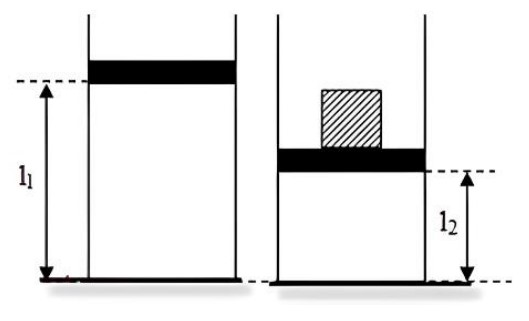
\includegraphics[scale=0.4]{../figs/FINAL-SEM1-002-5}}
	\shortans[oly]{226}
	\loigiai{
		\begin{center}
			\begin{tabular}{|M{5cm}|M{5cm}|M{5cm}|}
				\hline
			$p$&$V$ & $T$\\
			\hline
			$p_0=\SI{101325}{\pascal}$ & $60S$ & $30+273=\SI{303}{\kelvin}$\\
			\hline
			$p_0+\dfrac{F}{S}=\SI{151325}{\pascal}$ & $30S$ & $T_2$\\
			\hline
			\end{tabular}
		\end{center}
		$$\dfrac{p_1V_1}{T_1}=\dfrac{p_2V_2}{T_2}\Rightarrow T_2=\SI{226}{\kelvin}.$$
	}
\end{ex}
% ===============================================================
\begin{ex}
\immini{	Có ba bình thể tích $V_1=V$, $V_2=2V$, $V_3=3V$, thông với nhau nhưng cách nhiệt đối với nhau và với môi trường bên ngoài. Ban đầu các bình chứa khí ở cùng nhiệt độ $T_0$ và áp suất $p_0=\SI{1}{atm}$. Người ta giữ nguyên nhiệt độ bình 1, nâng nhiệt độ  bình 2 lên $2T_0$ và bình 3 lên $3T_0$. Áp suất mới trong các bình bằng bao nhiêu $\si{atm}$?}
{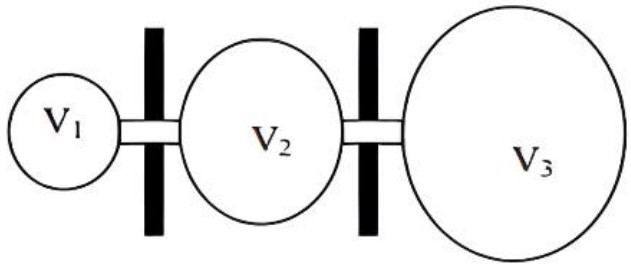
\includegraphics[scale=0.4]{../figs/FINAL-SEM1-002-6}}
	\shortans[oly]{2}
	\loigiai{
		$n=n_1+n_2+n_3\Leftrightarrow \dfrac{p_06V}{T_0}=\dfrac{pV}{T_0}+\dfrac{p\cdot 2V}{2T_0}+\dfrac{p\cdot 3V}{3T_0}\Rightarrow p=\SI{2}{atm}.$
	}
\end{ex}
\Closesolutionfile{ans}
\begin{center}
	\textbf{--- HẾT ---}
\end{center}
